A continuación, se presenta la estructura dialógica en los textos visuales seleccionados, así como la identificación sistemática de las escenas que agrupan símbolos, signos denotativos, anacronismos e imágenes-síntoma. Se desarrolla la metodología indicada, se muestra la imagen seleccionada, se incluye un párrafo descriptivo y se lleva a cabo la categorización de los elementos visuales presentes en la imagen. \textcolor{edit30sept}{Con el fin de consolidar el tránsito entre el análisis y la creación de exteriencia digital interactiva, se organiza el conjunto mediante una \textit{meta-composición estética y documental}. Esta operación de segundo orden integra descripción, categorización, montaje y reescritura escénica del \textit{corpus}, de modo que cada figura y su \textit{verbatim} constituyen nodos de una composición que reflexiona sobre su propio proceso documental y estético.}

Desde una perspectiva académica, es importante explicar que el análisis de imágenes presentado en este estudio evita deliberadamente establecer conclusiones definitivas por varias razones metodológicas y epistemológicas fundamentales. \textcolor{edit30sept}{Esta apertura epistémica se corresponde con la intención de no clausurar el sentido, sino escenificar su emergencia a través de cuadros, anacronismos e \textit{imágenes-síntoma},} y así, reconocer que las imágenes poseen una naturaleza dialéctica y anacrónica que resiste las interpretaciones unívocas. Las imágenes, como síntomas de procesos sociales e históricos complejos, demandan una aproximación que privilegie la apertura interpretativa por sobre la clausura del sentido, busca generar conocimiento a través de la yuxtaposición y el diálogo entre imágenes, más que mediante la imposición de significados predeterminados.

Dada la naturaleza sensible del caso del Hospital San Juan de Dios y la implicación personal del investigador, el estudio adopta una postura ética que evita la pretensión de objetividad absoluta. En su lugar, propone un acercamiento poético que:

\begin{enumerate}
    \item Reconoce la subjetividad inherente a toda interpretación.
    \item Invita al lector/espectador a participar activamente en la construcción de significado.
    \item Preserva la complejidad y multidimensionalidad del fenómeno estudiado.
\end{enumerate}

Esta aproximación no busca establecer verdades definitivas sino generar un espacio de reflexión donde las imágenes actúen como mediadoras entre la experiencia histórica y la memoria colectiva, permitiendo que cada lectoautor complete el sentido desde su propia experiencia y emergencia del sentido de manera relacional.


\clearpage
\begin{figure}[h!]
    \centering
    \includegraphics[width=\textwidth]{AlaDeriva_diaz2016_fotograma-00-34-25.png}
    \caption{AlaDeriva diaz2016 fotograma 00:34:25}
    \label{fig:AlaDeriva_diaz2016_fotograma_00_34_25}
\end{figure}

Cocina de tamaño medio, con una ventana grande que ocupa casi toda una pared. La luz natural entra por la ventana, creando sombras y contrastes en los objetos. Una persona de espaldas cocinando en una estufa. Una mesa grande cubierta de objetos, incluyendo platos sucios, bolsas, botellas y papeles. En las paredes hay cuadros y utensilios de cocina colgados. Una mesa en primer plano llena de objetos. La encimera al fondo está llena de utensilios de cocina. \parencite[fotograma: 00:34:25]{AlaDerivaDiaz2016}

\small
\singlespacing \begin{verbatim}
    graph TD
    A[[Anacronismo]]
    B[[Imagen-Síntoma]]

    A --> A1[Desorden flotante]
    A --> A2[Objetos sin tiempo, sin uso]
    A --> A3[Caos en silencio]

    B --> B1[Acumulación de objetos]
    B --> B2[Salud mental]
\end{verbatim}
\normalsize

\clearpage
\begin{figure}[h!]
    \centering
    \includegraphics[width=\textwidth]{Citytv_junio2015_fotograma-00-00-16.png}
    \caption{Citytv junio2015 fotograma 00:00:16}
    \label{fig:Citytv_junio2015_fotograma_00_00_16}
\end{figure}

Fachada de un edificio con el letrero `ORTESIS Y PROTESIS'. Hay dos ventanas visibles: una parcialmente cubierta con plástico y una prenda blanca colgando, mientras que la otra tiene una tela clara con patrones color azul. Un cintillo de noticias rojo indica: "San Juan de Dios será entregado en tres fases" y "Distrito satisfecho tras la adquisición", mostrando además la hora 7:31 y los valores del dólar y el euro. Algunas personas aparecen parcialmente visibles en la esquina inferior izquierda. \parencite[fotograma: 00:00:16]{CitytvJunio2015}

\small
\singlespacing \begin{verbatim}
    graph TD
    A[[Anacronismo]]
    B[[Imagen-Síntoma]]
    
    A --> A1[Susurra historias de servicios olvidados]
    A --> A2[Arquitectura que deplora]
    A --> A3[Afirmaciones oficiales subyacentes]
    
    B --> B1[Exteriorización de hábitad humano]
    B --> B2[Contraste frase optimista y entorno desgastado]
\end{verbatim}
\normalsize

\clearpage
\begin{figure}[h!]
    \centering
    \includegraphics[width=\textwidth]{AlaDeriva_diaz2016_fotograma-00-05-54.png}
    \caption{AlaDeriva diaz2016 fotograma 00:05:54}
    \label{fig:AlaDeriva_diaz2016_fotograma_00_05_54}
\end{figure}

Exterior del HSJD carrera décima vista hacia el sur. Se observa un vehículo blindado negro tipo antimotines con equipo de dispersión de agua en el techo. En primer plano, sobre el pavimento mojado, hay una persona vestida con bata blanca. Al fondo se distingue un grupo de policías con escudos antidisturbios formando una línea, mientras un chorro de agua es disparado hacia la derecha de la escena. \parencite[fotograma: 00:05:54]{AlaDerivaDiaz2016}

\small
\singlespacing \begin{verbatim}
    graph TD
    A[[Anacronismo]]
    B[[Imagen-Síntoma]]

    A --> A1[Vehículo moderno en calle tradicional, coexistencia de épocas]
    A --> A2[Antidisturbios contra el cuidado]
    A --> A3[Tensión social latente]

    B --> B1[Desigualdad y control policial en sociedad]
    B --> B2[Disturbios como síntoma de descontento actual]
\end{verbatim}
\normalsize

\clearpage
\begin{figure}[h!]
    \centering
    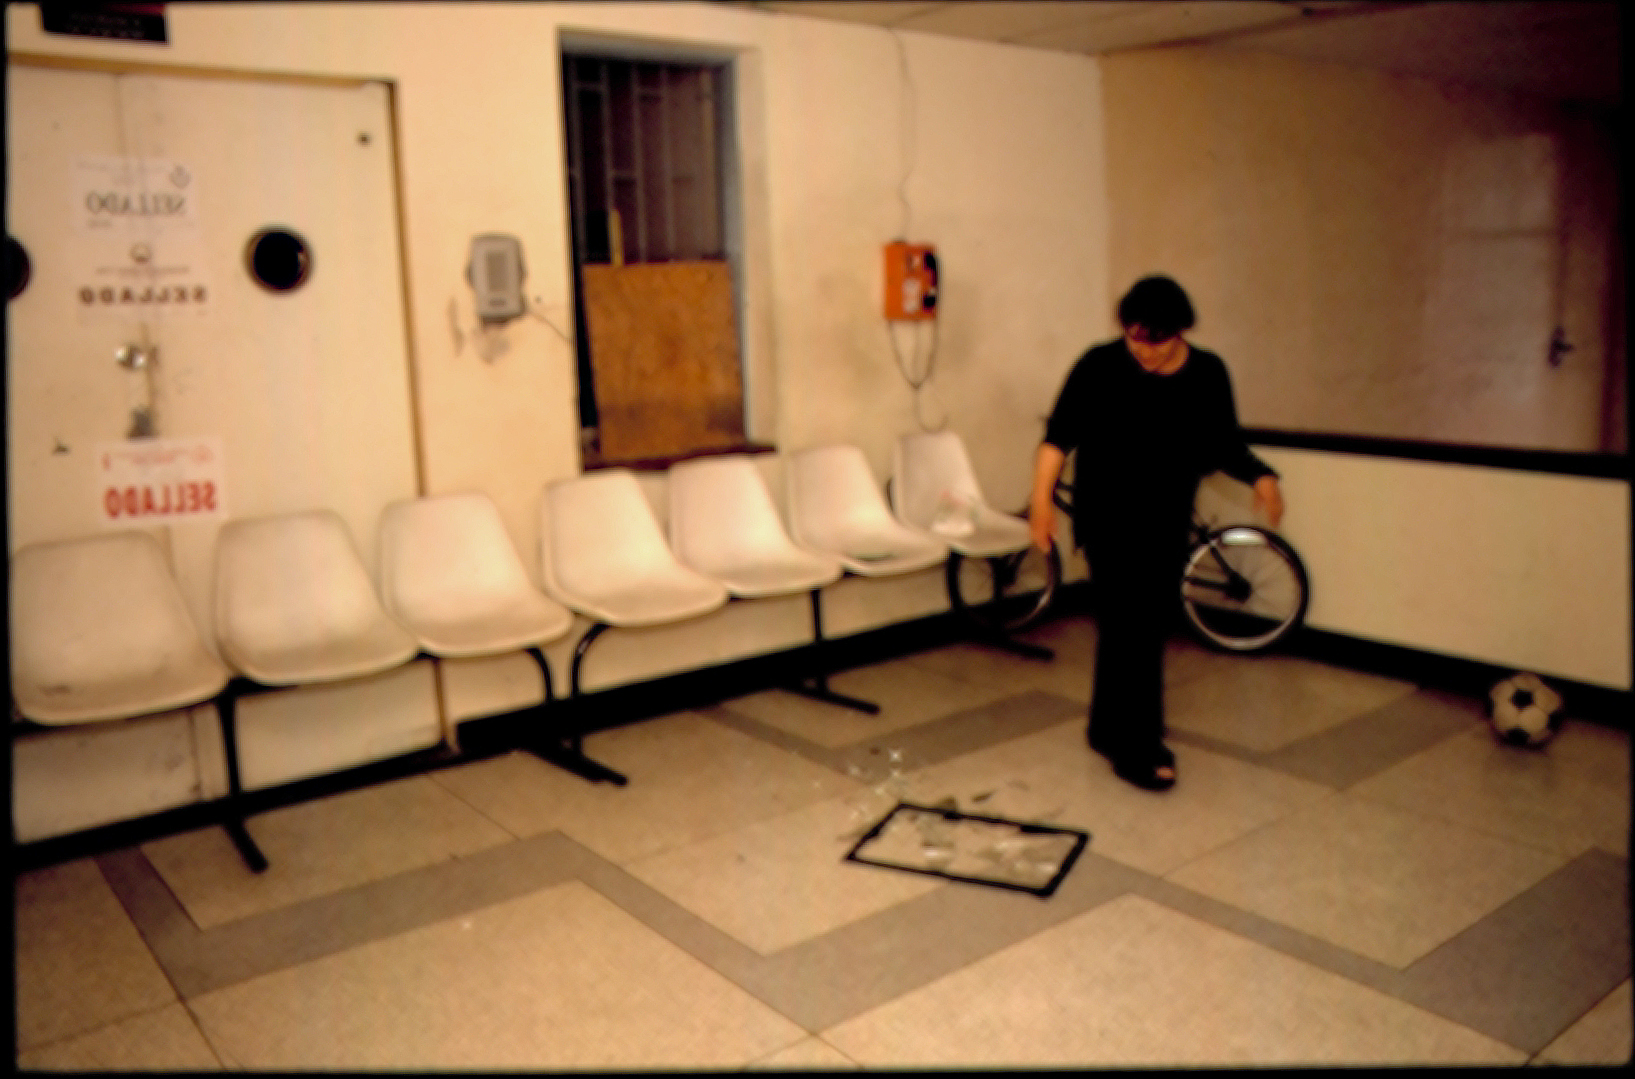
\includegraphics[width=\textwidth]{archivoMargarita_6octubre2004.jpg}
    \caption{Archivo Margarita 6 de octubre 2004}
    \label{fig:archivoMargarita_6octubre2004}
\end{figure}

Sala de espera con una fila de asientos blancos de plástico montados sobre una estructura metálica negra. La pared es de color crema claro con algunos elementos montados como un tablero y un teléfono naranja. El piso tiene un patrón geométrico en tonos beige y gris. En la escena hay una persona vestida de negro que mira hacia el suelo a lo que perece ser un marco y cristal rotos. Hay una bicicleta, un balón de fútbol y detrás de la hilera de sillas a la izquierda una puerta con letreros de `SELLADO'.

\small
\singlespacing \begin{verbatim}
graph TD
    A[[Anacronismo]]
    B[[Imagen-Síntoma]]
    
    A --> A1[Sala de espera vacía y austera]
    A --> A2[En tonos apagados]
    B --> A3[Lo lúdico se asoma]
    
    B --> B1[Soledad y aislamiento del individuo]
    B --> B2[Deshumanización en espacios institucionales]
\end{verbatim}
\normalsize

\clearpage
\begin{figure}[h!]
    \centering
    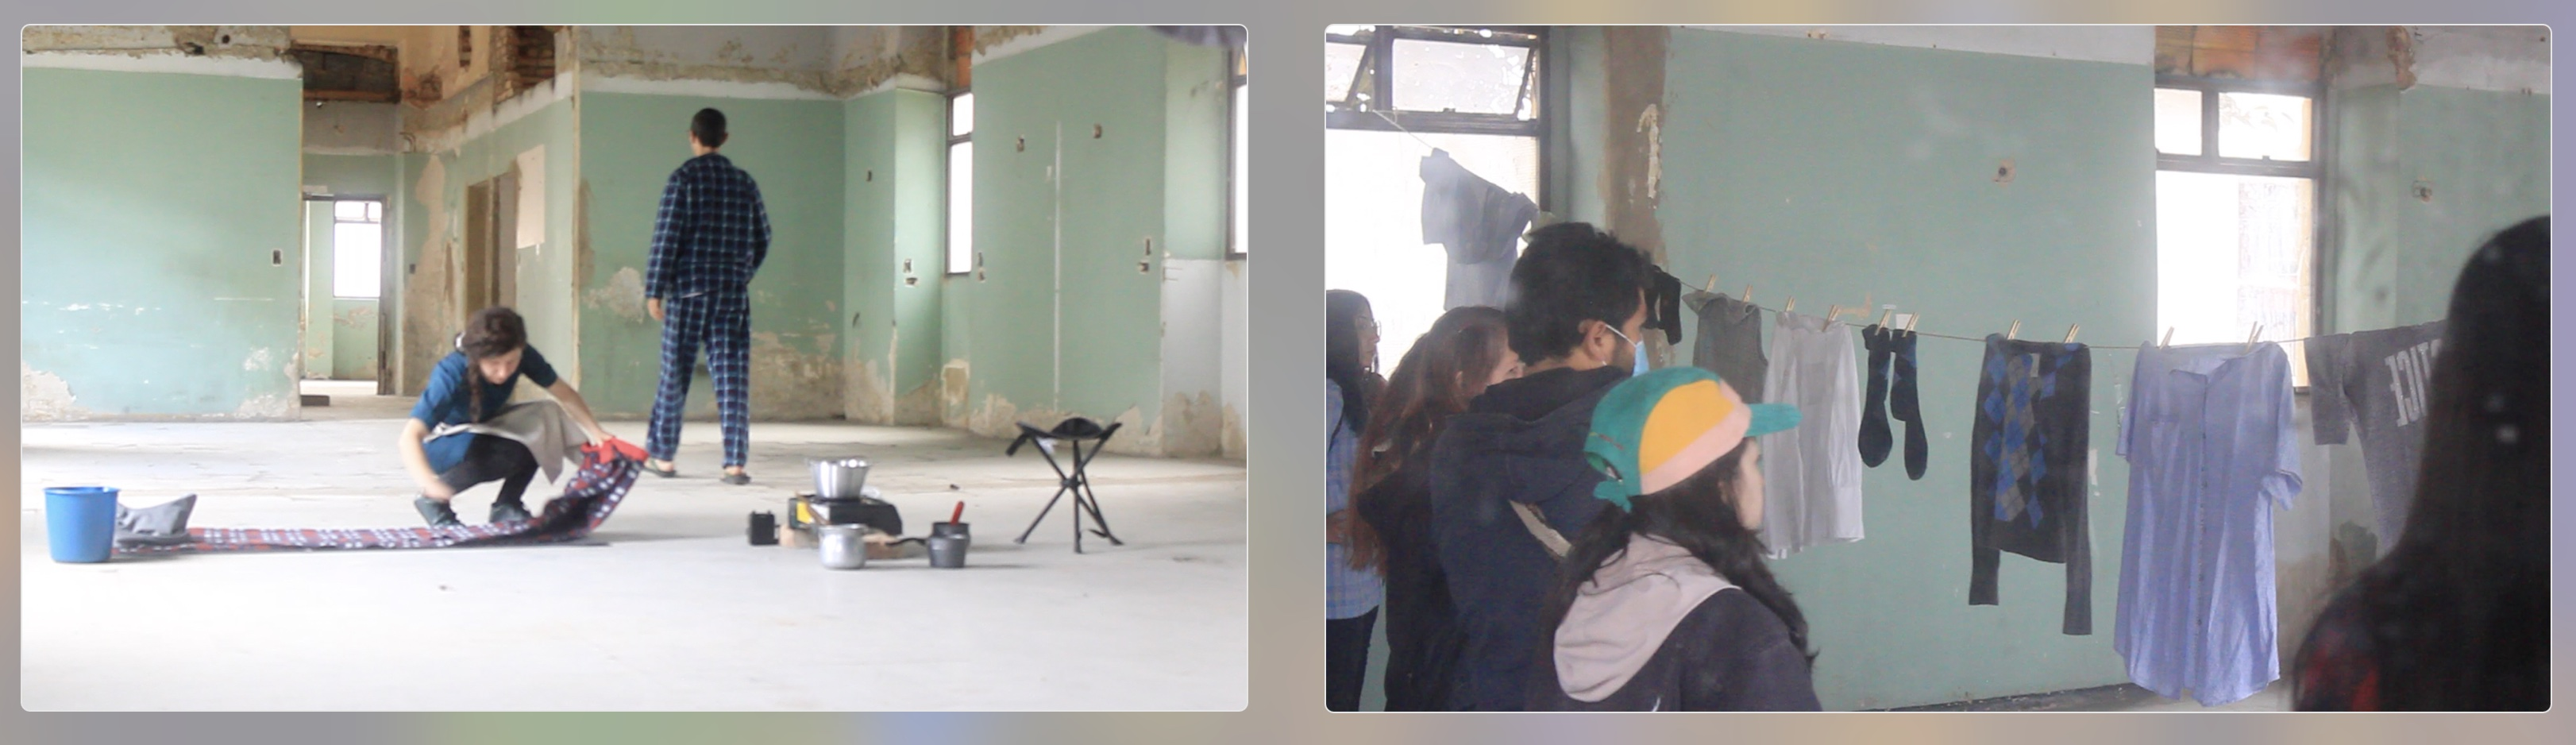
\includegraphics[width=\textwidth]{archivoJuanArroyo_10September2022_04_33.jpg}
    \caption{Archivo Juan Arroyo 10 de Septiembre 2022}
    \label{fig:archivoJuanArroyo_10September2022_04_33}
\end{figure}

\textit{Performance}. La imagen muestra edificio San Lucas en proceso de renovación o reparación. En la primera fotografía, se observan dos personas realizando tareas en el espacio - una sentada en el suelo trabajando con herramientas, y otra de pie observando. La segunda fotografía muestra a una persona sola de espaldas en el mismo espacio, se aprecia ropa colgada en una cuerda, dando la impresión de un espacio doméstico improvisado. Las paredes desgastadas, ventanas en crudo y suelo de concreto sugieren que el edificio está en una fase inacabada o de transición. Se yuxtaponen  escenas cotidianas de trabajo y vida dentro del entorno hospitalario.

\small
\singlespacing \begin{verbatim}
graph TD
    A[[Anacronismo]]
    B[[Imagen-síntoma]]

    A --> A1[San Lucas cambia]
    A --> A2[Ropa al viento susurra]
    A --> A3[Hogar casual]

    B --> B1[Personas habitando en contexto disruptivo]
    B --> B2[Ningún mobiliario]
\end{verbatim}
\normalsize

\clearpage
\begin{figure}[h!]
    \centering
    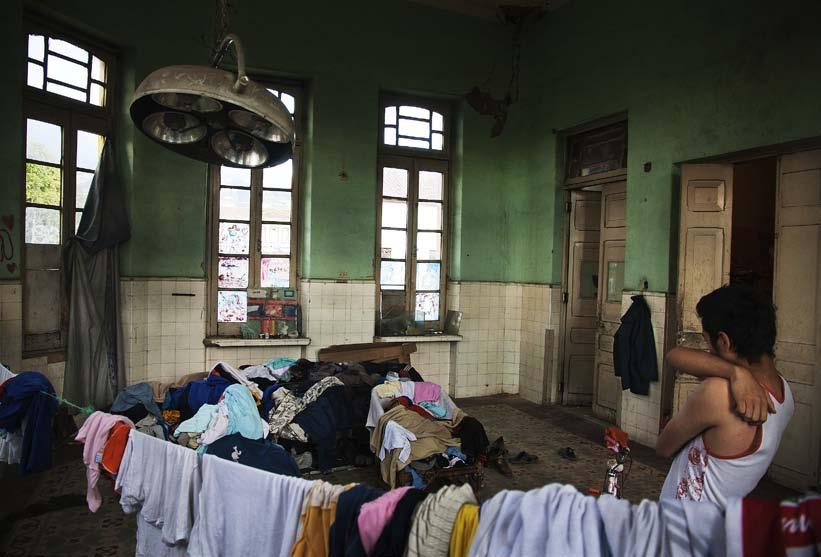
\includegraphics[width=\textwidth]{2011 Nicolas Van Hemelryck - San Juan sin Dios055.jpg}
    \caption{2011 Nicolas Van Hemelryck - San Juan sin Dios - 055}
    \label{fig:2011NicolasVanHemelryckSanJuansinDios-055}
\end{figure}

Sala de cirugía, interior deteriorado, ventanales que dejan entrar luz natural, contrastando con lámparas eléctricas colgantes. En este espacio se observan personas sentados en el piso sobre colchonetas y frazadas, rodeados de ropa y objetos personales. La escena revela síntomas de de usos disruptivos de ambiente para el cuidado quirúrjico y en hábitat doméstico. Foto del libro \parencite{Hemelryck2011}

\small
\singlespacing \begin{verbatim}
    graph TD
    A[[Anacronismo]]
    B[[Imagen-Síntoma]]

    A --> A1[Ventanas de otra era iluminan penumbras del presente]
    A --> A2[Despojos textiles de tiempos mezclados yacen inertes]
    A --> A3[Sombras del pasado acechan en la quietud actual]

    B --> B1[Abandono y precariedad se cuelan por los muros]
    B --> B2[Niñez expectante aguarda en silencio un futuro incierto]

\end{verbatim}
\normalsize


\clearpage
\begin{figure}[h!]
    \centering
    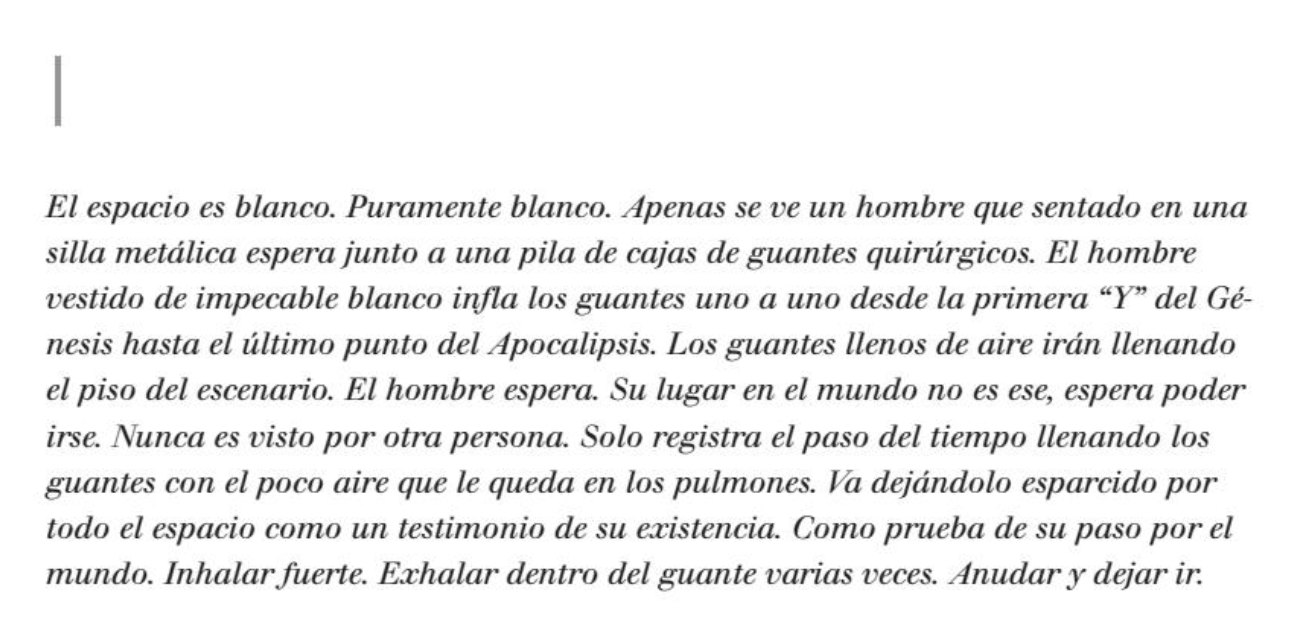
\includegraphics[width=\textwidth]{Ahumada2013_cuadro1.png}
    \caption{Cuadro I. Juan Camilo Ahumada, Tiempo de dios. 2013}
    \label{fig:Ahumada2013_cuadro1}
\end{figure}

\parencite[p. 10]{Ahumada2013}

\small
\singlespacing \begin{verbatim}
graph TD
    A[[Anacronismo]]
    B[[Imagen-Síntoma]]
    
    A --> A1[Impecabilidad atemporal y vacío]
    A --> A2[Guantes quirúrgicos y el aliento]

    B --> B1[Desconexión y falta de propósito]
    B --> B2[Automatización existencial]

\end{verbatim}
\normalsize

\clearpage
\begin{figure}[h!]
    \centering
    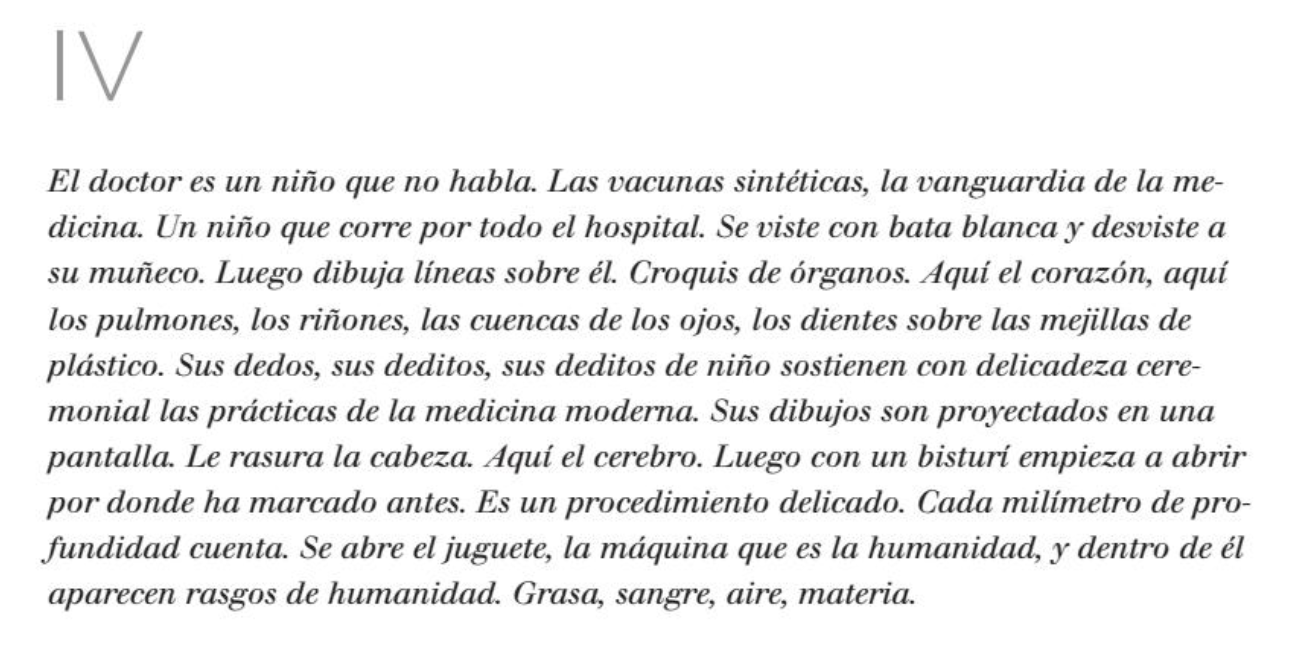
\includegraphics[width=\textwidth]{Ahumada2013_cuadro4.png}
    \caption{Cuadro IV. Juan Camilo Ahumada, Tiempo de dios. 2013}
    \label{fig:Ahumada2013_cuadro4}
\end{figure}

\parencite[p. 12]{Ahumada2013}

\small
\singlespacing \begin{verbatim}
    graph TD
    A[[Anacronismo]]
    B[[Imagen-Síntoma]]
    
    A --> A1[El doctor, un niño que no habla, cirugía moderna]
    A --> A2[Bata blanca y tecnología]
    A --> A3[La humanidad interna revelada]
    
    B --> B1[Avances médicos y fragilidad del cuerpo]
    B --> B2[Ética y cuidado humano]

\end{verbatim}
\normalsize


\clearpage
\begin{figure}[h!]
    \centering
    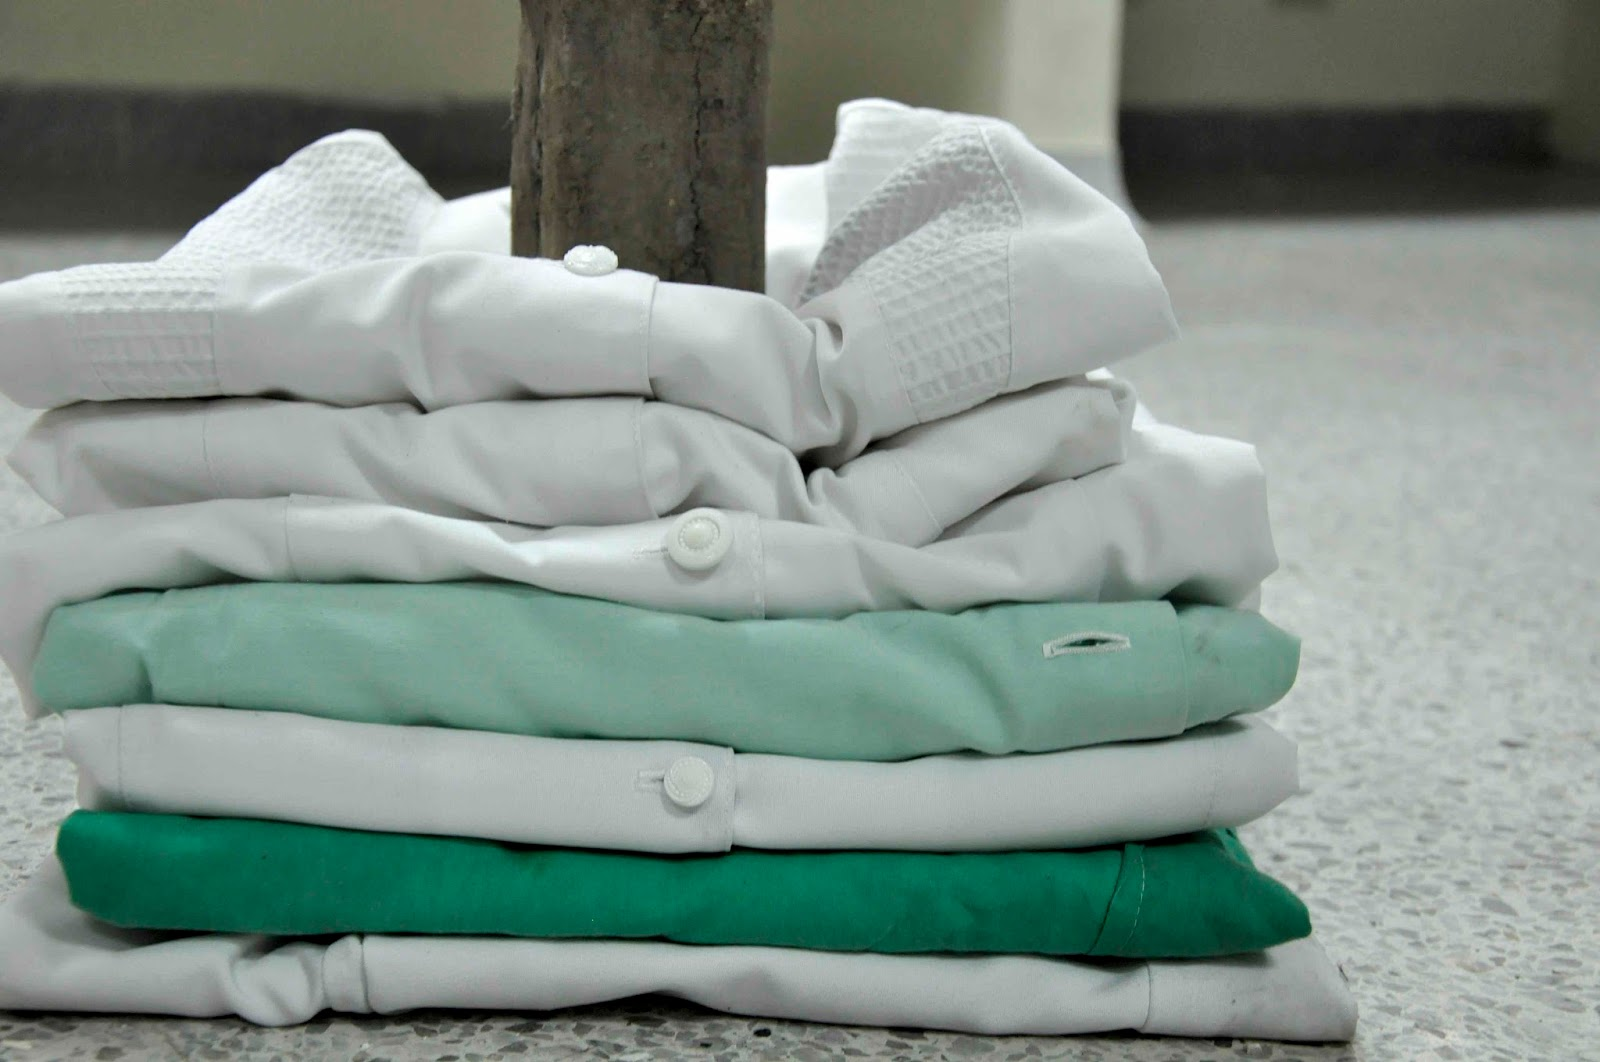
\includegraphics[width=\textwidth]{Una de las resistencias Karina Moreno 2015_5.jpg}
    \caption{\textit{Una de las resistencias} Ana Karina Moreno, 2015.}
    \label{fig:KarinaMoreno2015}
\end{figure}

Interior de edificio, postes de madera sosteniendo el techo sobre batas blancas y verdes apiladas. La tela se ve usada y pulcra, con arrugas y pliegues naturales.

\small
\singlespacing \begin{verbatim}
    graph TD
    A[[Anacronismo]]
    B[[Imagen-Síntoma]]
    
    A --> A1[Anhelo atemporal de pureza ]
    A --> A2[Contraste tela y rudeza natural]
    A --> A3[Ropa y pilar]

    B --> B1[Resistencia y fragilidad]

\end{verbatim}
\normalsize


\clearpage
\begin{figure}[h!]
    \centering
    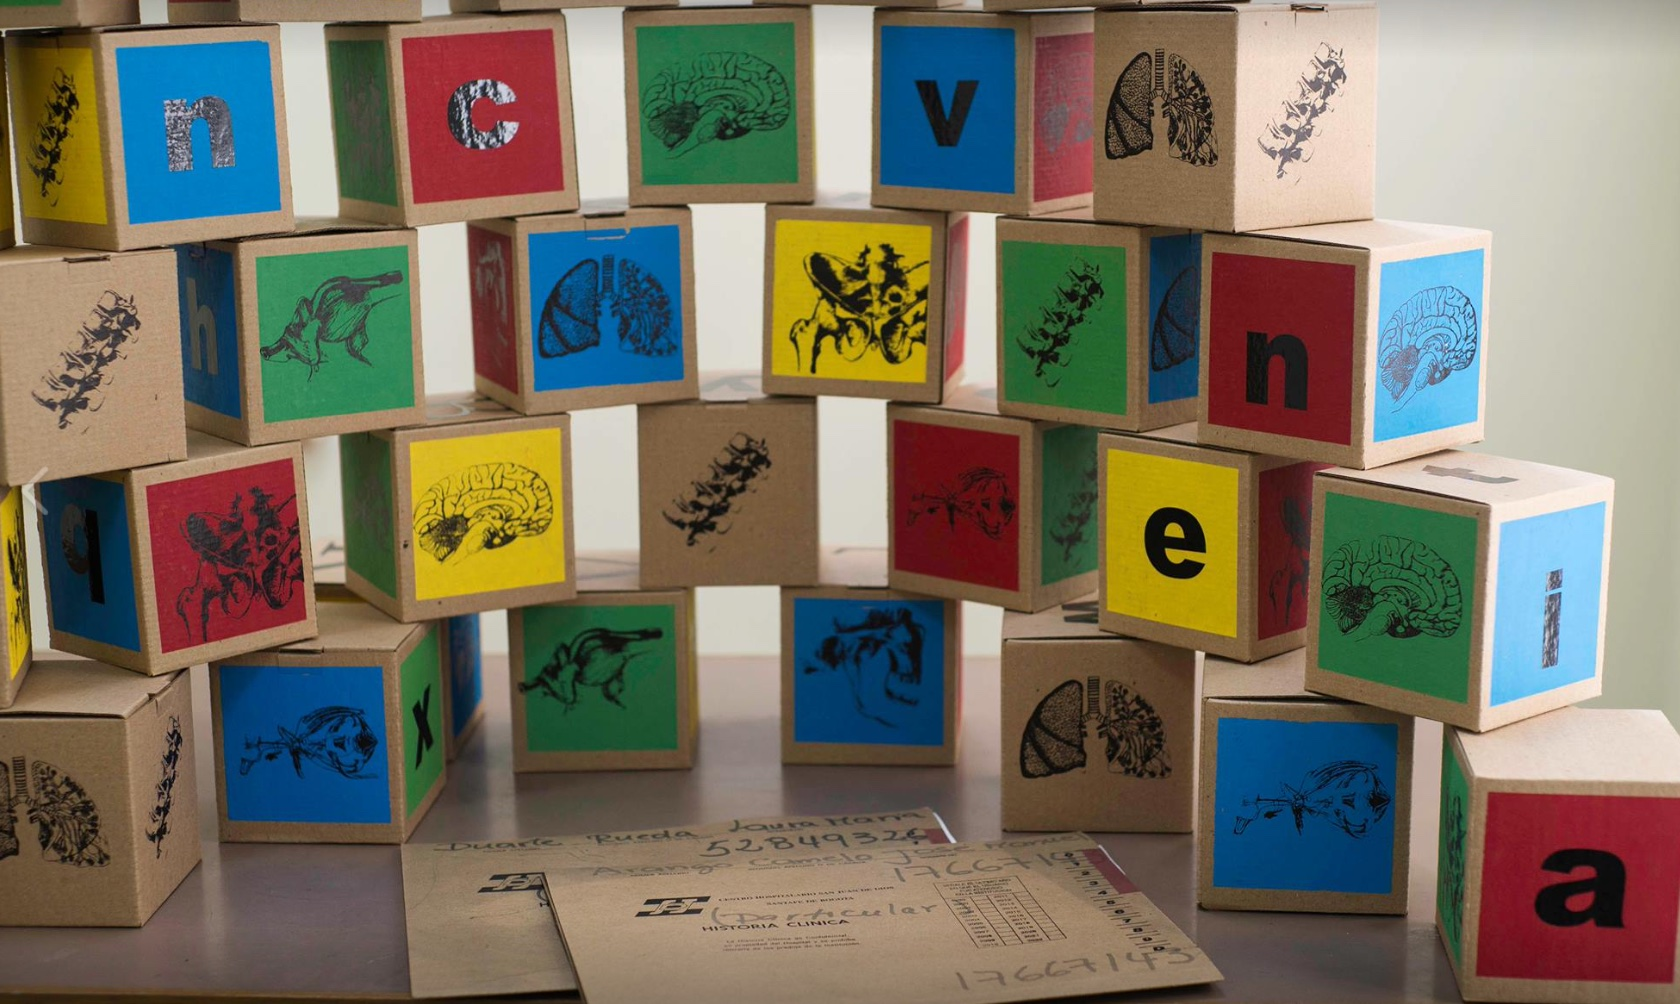
\includegraphics[width=\textwidth]{Duarte_didacticos.jpg}
    \caption{Didácticos para una sala de espera, Jenniffer Duarte 2015}
    \label{fig:JennifferDuarte2015}
\end{figure}

Colección de cubos apilados de madera, cada uno pintado con una letra del alfabeto y una ilustración en blanco y negro de diversos animales y partes del cuerpo humano, como cerebros y pulmones, en un estilo gráfico similar a grabados médicos antiguos. Sobres con hojas de historia clínica.

\small
\singlespacing \begin{verbatim}
    graph TD
    A[[Anacronismo]]
    B[[Imagen-Síntoma]]

    A --> A1[Bloques de juguete y grabados de ciencia]
    A --> A2[Lúdico infantil y la anatomía clásica]
    A --> A3[Fascinación perenne por el cuerpo]

    B --> B1[Alfabetización visual y biología humana]
    B --> B2[Curiosidad y asombro]
\end{verbatim}
\normalsize

\clearpage
\begin{figure}[h!]
    \centering
    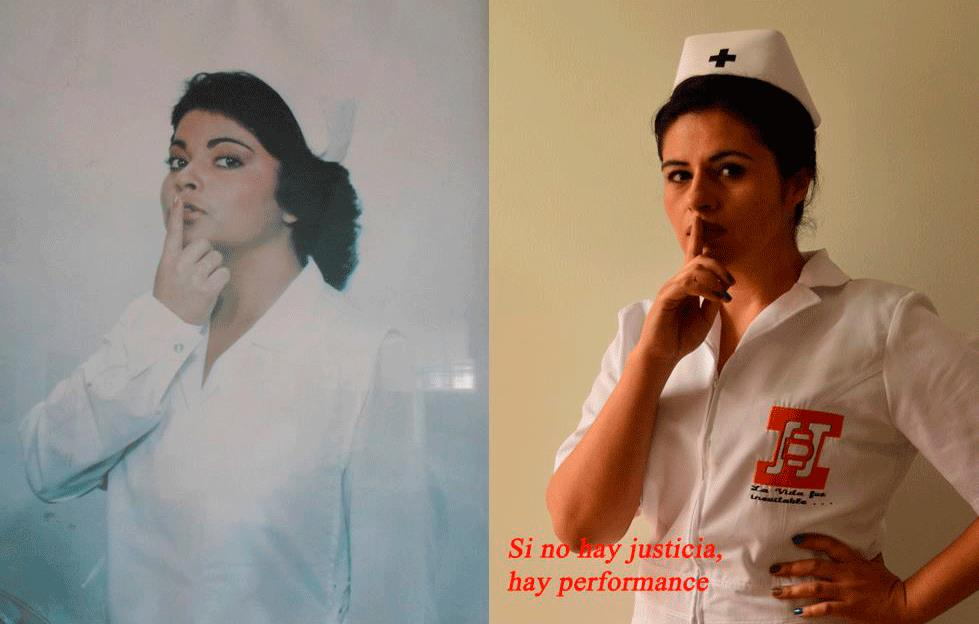
\includegraphics[width=\textwidth]{si no hay justicia hay performance.jpg}
    \caption{2016 Luisa Fernanda Vela - Al margen}
    \label{fig:LuisaVela2016}
\end{figure}

El montaje fotográfico yuxtapone dos retratos en blanco y negro de mujeres jóvenes de épocas distintas. A la izquierda, una imagen antigua muestra una mujer con peinado y ropa de los años 50, mirando pensativa con un dedo en los labios. A la derecha, una imagen contemporánea presenta una mujer con uniforme de enfermera y gesto serio, con la mano en la barbilla en actitud reflexiva. Debajo, un texto en español conecta ambas imágenes: ``Si no hay justicia, hay performance''.

\small
\singlespacing \begin{verbatim}
    graph TD
    A[[Anacronismo]]
    B[[Imagen-Síntoma]]

    A --> A1[Moda y peinados de distintas décadas se encuentran]
    A --> A2[Actitud contemplativa perdura a través del tiempo]
    A --> A3[Anhelo de justicia late en poses de mujeres pensativas]

    B --> B1[Mujeres en roles tradicionales cuestionan su realidad]
    B --> B2[Gesto meditativo surge ante injusticias presentes]
\end{verbatim}
\normalsize